\chapter{エントロピーと情報}

\begin{ex}
    \label{ex11.1}
    2値エントロピー$H(p,1-p)$とすると,
    \begin{align*}
        H\left(p,1-p\right) \leq H\left(\frac{1}{2}, \frac{1}{2}\right)
    \end{align*}
\end{ex}

\begin{ex}
    \label{ex11.2}
    まず, 関数方程式
    \begin{align*}
        f(x+y) = f(x) + f(y)
    \end{align*}
    を満たす連続関数が, 定数$a$を用いて, $f(x) = ax$であることを言う. 関数方程式より,
    \begin{align*}
        f(x) & = - f(-x)                     \\
        f(n) & = nf(1) \  (n \in \mathbb{N})
    \end{align*}
    なので, 任意の整数$m$に対して,
    \begin{align*}
        f(m) = f(1) m.
    \end{align*}
    また, 任意の自然数$n$, 任意の整数$m$に対して,
    \begin{align*}
        f\left( \frac{m}{n}\right) =  \frac{1}{n} f(m) = \frac{m}{n} f(1)
    \end{align*}
    つまり, 任意の有理数$x$に対して,
    \begin{align*}
        f(x) = f(1)x.
    \end{align*}
    $f$は連続なので, 任意の実数$x$に対して,
    \begin{align*}
        f(x) = f(1) x.
    \end{align*}
    \par
    $a >1, x,y < 0$に対して, $I$が,
    \begin{align*}
        I ( a^{x+y}) = I(a^x) + I(a^y)
    \end{align*}
    を満たすとすると, 上に示したことから,
    \begin{align*}
        I(a^x) = I(a) x
    \end{align*}
    が言えるので, $0 < p = a^x \leq 1$として,
    \begin{align*}
        I(p) = I(a) \log_a p.
    \end{align*}
\end{ex}

\begin{ex}
    \label{ex11.3}
    演習\ref{ex11.4}で示す, $H_{bin}(p)$の凹性と,
    \begin{align*}
        0 = \frac{d H_{bin}(p)}{dp} = \log \frac{1-p}{p}
        \longrightarrow p = \frac{1}{2}
    \end{align*}
    より, $H_{bin}(p)$の最大値は,
    \begin{align*}
        H_{bin} \left( \frac{1}{2}\right) = 1.
    \end{align*}
\end{ex}

\begin{ex}
    \label{ex11.4}
    \begin{align*}
        \frac{d^2 H_{bin}(p)}{d^2p} = - \frac{1}{p(1-p)} < 0.
    \end{align*}
\end{ex}

\begin{ex}
    \label{ex11.5}
    \begin{align*}
        H \left( p_{X,Y}(x,y) || p_X(x)p_Y(y) \right)
         & =
        - H\left(p_{X,Y}(x,y) \right) - \sum_{x,y} p_{X,Y}(x,y) \log \left[ p_X(x) p_Y(y)\right] \\
         & =
        - H\left(p_{X,Y}(x,y) \right)
        - \sum_{x,y} p_{X,Y}(x,y) \log p_X(x)
        - \sum_{x,y} p_{X,Y}(x,y) \log p_Y(y)
        \\
         & =
        - H\left(p_{X,Y}(x,y) \right)
        - \sum_{x} p_{Y}(y) \log p_X(x)
        - \sum_{y} p_{Y}(y) \log p_Y(y)
        \\
         & =
        - H(X,Y) + H(X) + H(Y)
    \end{align*}
    であることと定理11.1より,
    \begin{align*}
        H(X,Y) \leq H(X) + H(Y)
    \end{align*}
    が成立し, 等号成立は,
    \begin{align*}
        p_{X,Y}(x,y) = p_X(x) p_Y(y).
    \end{align*}
\end{ex}

\begin{ex}
    \label{ex11.6}
    (11.23)式より,
    \begin{align*}
        H(X, Y) = H(Y) - \sum_{x,y}p_{X,Y}(x,y) \log p_{X|Y}(x|y).
    \end{align*}
    また,
    \begin{align*}
        H(X,Y,Z)
         & = - \sum_{x,y,z} p_{X,Y,Z}(x,y,z)\log  p_{X,Y,Z}(x,y,z)                           \\
         & = - \sum_{x,y,z} p_{X,Y,Z}(x,y,z)\log \left[ p_{X|Y,Z}(x|y,z) p_{Y,Z}(y,z)\right] \\
         & = H(Y,Z) - \sum_{x,y,z} p_{X,Y,Z}(x,y,z)\log p_{X|Y,Z}(x|y,z).
    \end{align*}
    ゆえに,
    \begin{align*}
         & H(X,Y,Z) - H(Y,Z) - H(X,Y) + H(Y)                                       \\
         & =
        - \sum_{x,y,z} p_{X,Y,Z}(x,y,z)\log p_{X|Y,Z}(x|y,z)
        + \sum_{x,y}p_{X,Y}(x,y) \log p_{X|Y}(x|y)                                 \\
         & =
        \sum_{x, y, z}  p_{X,Y,Z}(x,y,z)\log \frac{p_{X|Y}(x|y)}{p_{X|Y,Z}(x|y,z)} \\
         & \leq
        \frac{1}{\ln2}\sum_{x, y, z}  p_{X,Y,Z}(x,y,z)
        \left( \frac{p_{X|Y}(x|y)}{p_{X|Y,Z}(x|y,z)} - 1 \right)                   \\
         & =
        \frac{1}{\ln2} \left( \sum_{x, y, z} p_{Y,Z}(y,z) p_{X|Y}(x|y) - 1 \right) \\
         & =
        \frac{1}{\ln2} \left( \sum_{x, y} p_{Y}(y) p_{X|Y}(x|y) - 1 \right)        \\
         & =
        \frac{1}{\ln2} \left( \sum_{x} p_{X}(x) - 1 \right) = 0.
    \end{align*}
    等号成立は,
    \begin{align*}
        p_{X|Y}(x|y) = p_{X|Y,Z}(x|y,z)
    \end{align*}
    つまり, $Z \to Y \to X$がMarkov chainをなすとき.
\end{ex}

\begin{ex}
    \label{ex11.7}
\end{ex}

\begin{ex}
    \label{ex11.8}
    \begin{align*}
        H(X, Y : Z) = 1, H(X:Z) = H(Y:Z) = 0.
    \end{align*}
\end{ex}

\begin{ex}
    \label{ex11.9}
    \begin{align*}
        H(X_1 : Y_1) = H(X_2 : Y_2) =  H(X_1, X_2 : Y_1, Y_2) = 1.
    \end{align*}
\end{ex}

\begin{ex}
    \label{ex11.10}
    \begin{align*}
        X \to Y \to Z \mathrm{がMarkov\ chainをなす}
         & \longrightarrow
        P_{Z|X,Y}(z|x,y) = p_{Z|Y}(z|y)                                       \\
         & \longrightarrow
        \frac{p_{X,Y,Z}(x,y,z)}{p_{X,Y}(x,y)} = \frac{p_{Y,Z}(y,z)}{p_{Y}(y)} \\
         & \longrightarrow
        \frac{p_{X,Y,Z}(x,y,z)}{p_{Y,Z}(y,z)} = \frac{p_{X,Y}(x,y)}{p_{Y}(y)} \\
         & \longrightarrow
        P_{X|Y,Z}(z|x,y) = p_{X|Y}(x|y)                                       \\
         & \longrightarrow
        Z \to Y \to X \mathrm{がMarkov\ chainをなす}
    \end{align*}
\end{ex}

\begin{ex}
    \label{ex11.11}
    \begin{align*}
        0,\ 0, \ H_{bin}\left( \frac{3 + \sqrt{5}}{6}\right).
    \end{align*}
\end{ex}

\begin{ex}
    \label{ex11.12}
    \begin{align*}
        D = \sqrt{1-2p(1-p)}
    \end{align*}
    として,
    \begin{align*}
        S\left( \rho\right) = H\left( \frac{1 + \sqrt{D}}{2}, \frac{1 - \sqrt{D}}{2}\right) \leq H(p,1-p).
    \end{align*}
    \begin{figure}[H]
        \begin{center}
            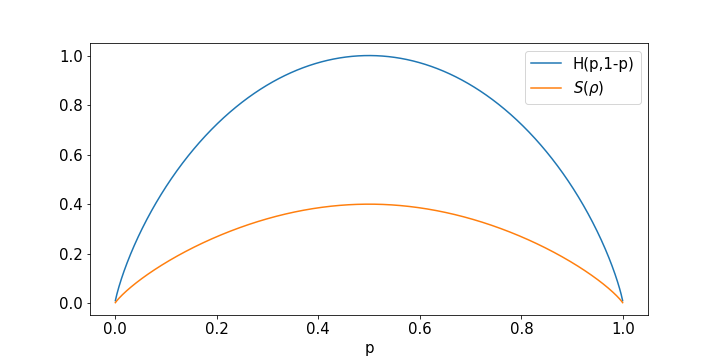
\includegraphics[width = 80mm]{./fig/ex11_12.png}
        \end{center}
    \end{figure}
\end{ex}

\begin{ex}
    \label{ex11.13}
    定理11.8(5)において,
    \begin{align*}
        \rho = \sum_i p_i \ket{i}\bra{i}, \rho_i = \sigma
    \end{align*}
    とすると,
    \begin{align*}
        S\left( \rho \otimes \sigma \right) = S(\rho) + S(\sigma).
    \end{align*}
    \par
    また,
    \begin{align*}
        \rho = \sum_i p_i \ket{i}\bra{i} \\
        \sigma = \sum_j q_j \ket{\tilde{j}}\bra{\tilde{j}}
    \end{align*}
    とすると,
    \begin{align*}
        \rho \otimes \sigma =
        \sum_{i,j} p_i q_j
        \left( \ket{i} \otimes \ket{\tilde{j}} \right)
        \left( \bra{i} \otimes \bra{\tilde{j}} \right)
    \end{align*}
    なので,
    \begin{align*}
        S\left( \rho \otimes \sigma \right) =
        -\sum_{ij} p_i q_j \log \left[ p_i q_j \right]
        =
        -\sum_{i} p_i \log p_i
        -\sum_{j} qol,_j \log q_j
        =
        S(\rho) + S(\sigma).
    \end{align*}
\end{ex}


\begin{ex}
    \label{ex11.14}
    \begin{align*}
        \ket{AB}\mathrm{が純粋状態}, S(B|A)<0
        \longleftrightarrow
        S(A) > 0
        \longleftrightarrow
        A \mathrm{が純粋状態でない}
        \longleftrightarrow
        \ket{AB}\mathrm{がもつれている}
    \end{align*}
    最後の$\longleftrightarrow$では,
    \begin{align*}
        \ket{AB}\mathrm{がもつれていない}
        \longleftrightarrow
        \ket{AB} = \ket{A} \otimes \ket{B}
        \longleftrightarrow
        \rho^A = \ket{A} \bra{A}
        \longleftrightarrow
        A\mathrm{が純粋状態}
    \end{align*}
    であることを用いた.
\end{ex}

\begin{ex}
    \label{ex11.15}
    測定後の状態$\rho'$は,
    \begin{align*}
        \rho'
        = M_1 \rho M_1^\dagger + M_2 \rho M_2^\dagger
        = \tr [\rho] \ket{0}\bra{0} = \ket{0}\bra{0}
    \end{align*}
    より, $S(\rho') = 0$であるから, $S(\rho) \geq S(\rho')$.
\end{ex}

\begin{ex}
    \label{ex11.16}
    $\rho^{AB}$は混合状態として.
    \begin{align*}
        \rho^{AB} = \sum \lambda_i \ket{i^{AB}} \bra{i^AB}
    \end{align*}
    とかくと,
    \begin{align*}
        \rho^A = \sum \lambda_i \rho^A_i,
        \rho^B = \sum \lambda_i \rho^B_i
    \end{align*}
    となる. また, $AB$の純粋化$ABR$は, $R$の正規直交基底$\{ \ket{i^R} \}$として,
    \begin{align*}
        \ket{ABR}  & = \sum_i \sqrt{\lambda_i} \ket{i^{AB}} \ket{i^R} \\
        \rho^{ABR} & =  \sum_{ij} \sqrt{\lambda_i \lambda_j}
        \ket{i^{AB}} \bra{j^{AB}} \otimes \ket{i^{R}} \bra{j^{R}}     \\
    \end{align*}
    とかけるので,
    \begin{align*}
        \rho^{AR} & =  \sum_{ij} \sqrt{\lambda_i \lambda_j}
        \tr_B \left[\ket{i^{AB}} \bra{j^{AB}} \right] \otimes \ket{i^{R}} \bra{j^{R}} \\
        \rho^{R}  & =  \sum_{i} \lambda_i \ket{i^{R}} \bra{i^{R}}
    \end{align*}
    を得る.
    \par
    以上より,
    \begin{align*}
         & \ \ \ \ \ \ \  S(A,B) = S(B) - S(A)
        \\
         & \longleftrightarrow
        \rho^{AR} = \rho^A \otimes \rho^R
        \\
         & \longleftrightarrow
        \sum_{ij} \lambda_i \lambda_j \rho_i^A \otimes \ket{j^R}\bra{j^R}
        =
        \sum_{ij} \sqrt{\lambda_i \lambda_j}
        \tr_B \left[\ket{i^{AB}} \bra{j^{AB}} \right] \otimes \ket{i^{R}} \bra{j^{R}}
        \\
         & \longleftrightarrow
        \tr_B \left[\ket{i^{AB}} \bra{j^{AB}} \right] = \delta_{ij} \rho_i^A
        \mathrm{\ \ \ かつ\ \ \ }
        \sum_{ij} \lambda_i \lambda_j \rho_i^A \otimes \ket{j^R} \bra{j^R}
        = \sum_i \lambda_i \rho_i^A \otimes \ket{i^R} \bra{i^R}
        \\
         & \longleftrightarrow
        \tr_B \left[\ket{i^{AB}} \bra{j^{AB}} \right] = \delta_{ij} \tr_B \left[ \ket{i^{AB}} \bra{i^{AB}} \right]
        \mathrm{\ \ \ かつ\ \ \ }
        \sum_{ij} \lambda_i \lambda_j \rho_i^A \otimes \ket{j^R} \bra{j^R}
        = \sum_{ij} \lambda_i \lambda_j \rho_j^A \otimes \ket{j^R} \bra{j^R}
        \\
         & \longleftrightarrow
        \{ \rho_i^B \} \mathrm{が互いに直交する台を持つ}
        \mathrm{\ \ \ かつ\ \ \ }
        \exists \rho \ \forall i \in \{ i \ |\  \lambda_i > 0 \} \ \rho_i = \rho
    \end{align*}
    最後の行の2つ目の主張については, \ref{ex11.18}で示す.
\end{ex}

\begin{ex}
    \label{ex11.17}
\end{ex}

\begin{ex}
    \label{ex11.18}
    示すべきは,
    \begin{align*}
        \sum_{ij} p_i p_j \rho_i \otimes \ket{j}\bra{j}
        =
        \sum_{j} p_j \rho_j \otimes \ket{j}\bra{j}
        \longleftrightarrow
        \exists \rho \ \forall i \in \{ i \ |\  p_i > 0 \} \ \rho_i = \rho
    \end{align*}
    \par
    $\longrightarrow)$
    \begin{align*}
        \sum_{ij} p_i p_j \rho_i \otimes \ket{j}\bra{j}
        =
        \sum_{j} p_j \rho_j \otimes \ket{j}\bra{j}
        =
        \sum_{ij} p_i p_j \rho_j \otimes \ket{j}\bra{j}
    \end{align*}
    であり, 両辺の系Bに対する部分とレースを取ると,
    \begin{align*}
        \sum_{ij} p_i p_j (\rho_i - \rho_j) = 0
    \end{align*}
    なので, $p_i > 0$なる任意の$i$の状態$\rho_i$は全て等しい.
    \par
    $\longleftarrow)$
    明らか.
\end{ex}


\begin{ex}
    \label{ex11.19}

    \begin{align*}
        S \left( \frac{I}{d}\right)
        =
        S \left( \sum_i p_i U_i \rho U_i^\dagger \right)
        \geq
        \sum_i p_i S \left( U_i \rho U_i^\dagger \right)
        =
        \sum_i p_i S\left( \rho \right)
        =
        S\left( \rho \right)
    \end{align*}
    で等号は,
    \begin{align*}
        \rho = \frac{I}{d}
    \end{align*}
    で成立. ここで, ユニタリ$U$に対して,
    \begin{align*}
        S \left( U \rho U^\dagger \right)
        =
        - \tr \left[ U \rho U^\dagger \log U \rho U^\dagger\right]
        =
        - \tr \left[ U \rho U^\dagger U (\log \rho) U^\dagger\right]
        =
        - \tr \left[ \rho \log \rho\right]
        =
        S \left( \rho\right)
    \end{align*}
    が成り立つことを用いた.
\end{ex}

\begin{ex}
    \label{ex11.20}
\end{ex}

\begin{ex}
    \label{ex11.21}
    $[ \rho , \sigma] = 0$とすると, これらは同時対角化可能で,
    \begin{align*}
        \rho = \sum_i p_i \ket{i} \bra{i},
        \sigma = \sum_i q_i \ket{i} \bra{i}
    \end{align*}
    とすると, von Neumannエントロピーの凹性より, $0 \le \lambda \le 1$に対して,
    \begin{align*}
        H( \{ \lambda p_i + (1 - \lambda) q_i\})
         & =
        - \sum_{i} \left( \lambda p_i + (1 - \lambda) q_i \right) \log \left( \lambda p_i + (1 - \lambda) q_i \right)
        \\
         & =S( \lambda \rho + (1 - \lambda) \sigma)
        \\
         & \geq
        \lambda S (\rho) + (1- \lambda) S(\sigma)
        \\
         & =
        \lambda H (\{ p_i \}) + (1- \lambda) H(\{ q_i\})
    \end{align*}
    と, Shannonエントロピーの凹性を示せた.
\end{ex}

\begin{ex}
    \label{ex11.22}
    $[ \rho , \sigma] = 0$とすると, これらは同時対角化可能で,
    \begin{align*}
        \rho = \sum_i p_i \ket{i} \bra{i},
        \sigma = \sum_i q_i \ket{i} \bra{i}
    \end{align*}
    とすると,
    \begin{align*}
        f(p)
        = S(p \rho + (1-p)\sigma)
        = - \sum_i
        \left[ \left( p_i - q_i \right) p + q_i \right]
        \log \left[  \left( p_i - q_i \right) p + q_i \right]
    \end{align*}
    なので, 
    \begin{align*}
        f''(p) = - \sum_i \frac{ (p_i - q_i)^2 }{p_i p + (1-p)q_i} \leq 0.
    \end{align*}
\end{ex}